\section{Electronic properties}

The influence of phosphorus vacancy and substitution hydrogen in place of phosphorus vacancy tetrahedral site to electronic properties of material was investigated in the current work. The main disadvantage of LiFePO$_4$ and LiMnPO$_4$ is their poor electronic conductivity in the pure form. The carbon coating is used at the sample preparation stage to solve this problem and make material without band-gap in Fermi level. Thus, the improvement of electronic properties of material is a crucial aim of its preparation. It can be affected by hydroxyl group defects due to the charge compensation mechanism. 

Firstly, the influence of phosphorus vacancy on the electronic conductivity can be considered in density of states study (Fig.\ref{ris:0DOS})

\begin{figure}[ht]
\center{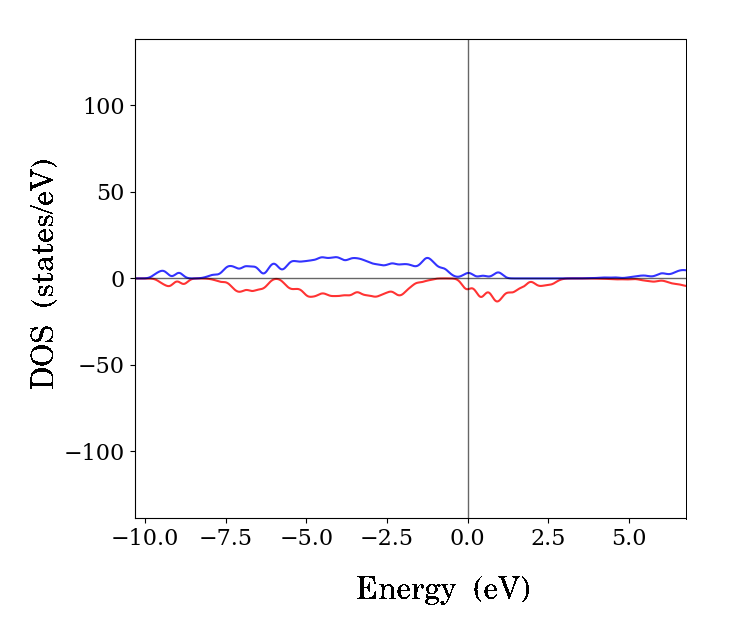
\includegraphics[width=0.9\linewidth]{pictures/0.png})}
\caption{Density of electronic states for LiFePO$_4$ with P$_{vacancy}$}
\label{ris:0DOS}
\end{figure}

The influence of 1, 2, 3 or 4 hydrogen substitution atom in place of defective PO$_4$ place is presented in Fig.\ref{ris:1-4DOS}. The absence of band-gap at the Fermi level is clearly seen. All of these defective materials are conductors.

\begin{figure}[ht]
\begin{minipage}[h]{0.5\linewidth}
\center{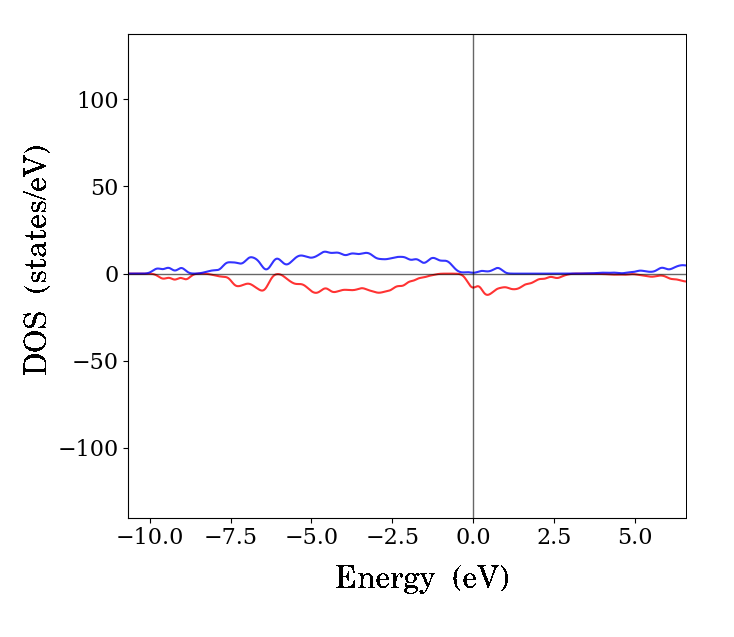
\includegraphics[width=1\linewidth]{pictures/1.png} \\ a) PO$_4$-O$_4$H }
\end{minipage}
\hfill
\begin{minipage}[ht]{0.5\linewidth}
\center{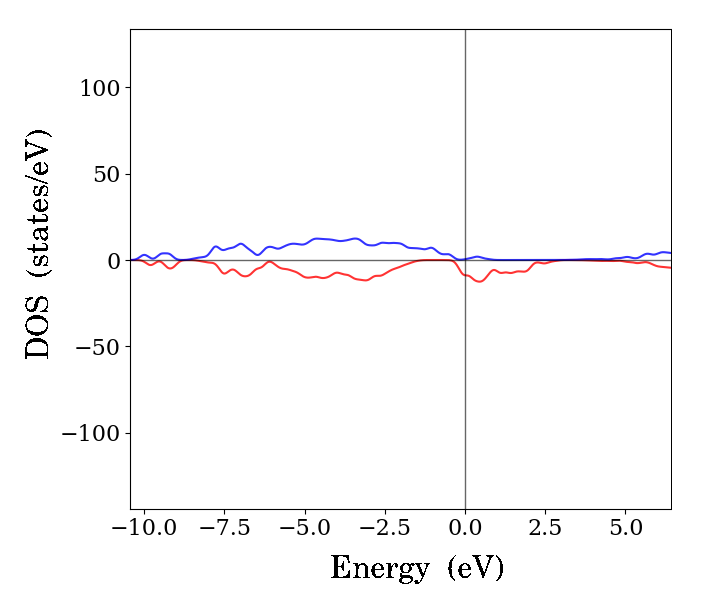
\includegraphics[width=1\linewidth]{pictures/2.png} \\ b) PO$_4$-O$_4$H$_2$ }
\end{minipage}
\vfill
\begin{minipage}[h]{0.5\linewidth}
\center{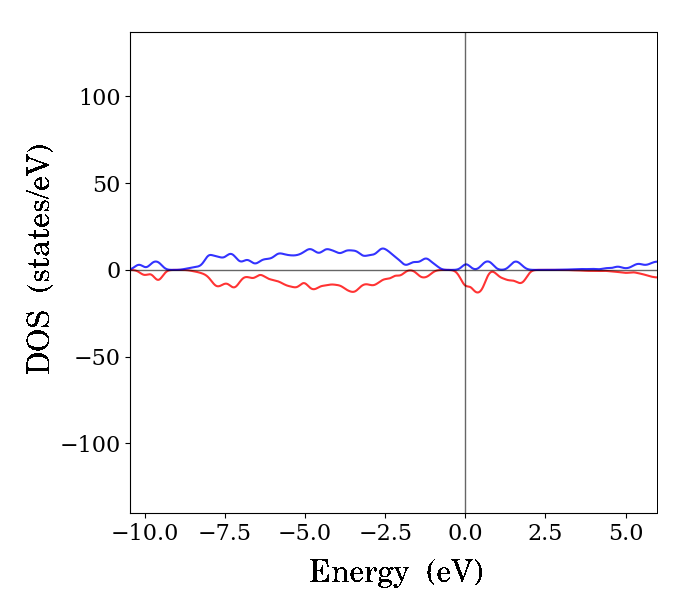
\includegraphics[width=1\linewidth]{pictures/3.png} \\ c) PO$_4$-O$_4$H$_2$ }
\end{minipage}
\hfill
\begin{minipage}[ht]{0.5\linewidth}
\center{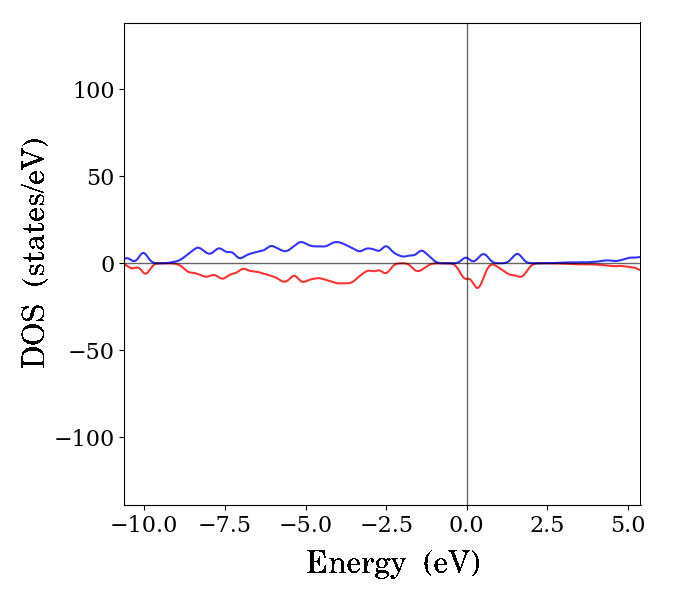
\includegraphics[width=1\linewidth]{pictures/4.png} \\ d) PO$_4$-O$_4$H$_4$ }
\end{minipage}
\caption{DOS of LiFePO$_4$ with different defect composition }
\label{ris:1-4DOS}
\end{figure}